\section{Umsetzung}\label{kap:ums}

\todo{Struktur Umsetzung einfügen }

\subsection{Parsen von Logikausdrücken}\label{kap:ums:parsing}
Das Ziel dieses Projektes ist es, dass die Ausgänge der Steuerung in Abhängigkeit von Eingängen wie physikalischen Eigängen oder zum Beispiel Timer-bausteinen ein beziehungsweise ausgeschaltet werden. Dafür ist in einer Textdatei für jeden Ausgang eine Zeile vorgesehen. Eine Zeile beginnt hierbei mit dem zu definierenden Ausgang, also zum Beispiel Ho1, worauf ein Gleichheitszeichen zu folgen hat. Der gesamte Ausdruck hinter dem Gleichheitszeichen wird zur Laufzeit des Programms durchlaufen, wobei jedes vorkommende Paar von [ und ] durch eine Null oder eine Eins ersetzt. Innerhalb der Klammern, findet sich gleich genau wie bei dem Bezeichner vor dem Gleichheitszeichen, die jeweilige Bezeichnung der Abhängigkeit. Lautet die Zeile also etwa Ho0= [Hi0] \& [Hi1] so wird die Komplette erste Klammer durch den Wert von Hi0 ersetzt, wärend die zweite Klammer  durch den Wert von Hi1 ersetzt wird. Daraus ergibt sich dann, vorausgesetzt Hi0 und Hi1 sind im Zustand \chphl{Ein}, Ho0= 1 \& 1. Das für den Leser offensichtliche Ergebnis dieser Gleichung ist 1 oder \chphl{true}. Jedoch gestaltet sich eine programmatische Lösung des Problems als deutlich komplexer. Denn sobald mehr als drei Ausdrücke im Spiel sind, müssen wie bei klassischer Mathematik Rechenregeln befolgt werden. Punkt vor Strich sowie die Beachtung von Klammern. Dabei kann ein Ausdruck beliebig Komplex sein. Eine Rechersche nach Ansätzen führte zu Stackoverflow.\cite{URL:Parsing} Dieser Ansatz löste genau das Problem und wurde somit in das Projekt übernommen. 
%
\subsection{Automatische Prüfung von Abhängigkeiten}\label{kap:ums:abh}
Ein Problem was sich mit dem Einbinden der Lösung zum Parsen der Logikausdrücke ergab, war die Abhängigkeit zu Boost. Auf dem Desktop Computer auf dem die Lösung getestet wurde, konnte das Projekt dank installiertem Boost Paket ohne Probleme übersetzt werden. Da es sich bei dem  Zielsystem jedoch um eine ARM Architektur handelt, musste der Programmcode dort Übersetzt werden. In den Paketquellen des dort installieren Raspbian, ist jedoch eine ältere Version des Boost Pakets hinterlegt, was dazu führt dass Boost manuell heruntergeladen und gebaut werden muss. Obwohl sich dieses Problem im Laufe der Zeit durch Aktualisierung des Paketes in den Paketquellen von Raspbian von selbst lösen wird, muss dennoch geprüft werden ob die installierte Version den Ansprüchen genügt. Hierfür wurde ein Bash-Script erstellt, welches auch alle weiteren Abhängigkeiten Prüft und gegebenenfalls installiert. Dazu zählen auch die im  \autoref{chp:anhang} aufgeführten Bibliotheken um die Hardware anzusprechen und der verwendete Kompiler. 
 
\subsection{Benamungsschnema}\label{kap:ums:banamsung}
Nachdem die Auswertung beziehungsweise das Parsing der Logikausdrücke funktionierte, sollte auch die Auswertung der Bezeichner automatisiert werden. Ein Benamsungsschema wurde dabei schon vorher erdacht. Es besteht aus einem führenden Großbuchstaben, gefolgt von einem Kleinbuchstaben und einer Zahl. Dabei wird der führende Buchstabe als Kanal bezeichnet, der zweite als Entität und die Ziffer als Pin-Nummer. So könnte zum Beispiel der Buchstabe \chphl{H} den Kanal Hardware beschreiben, welcher  wiederrum die Entitäten \chphl{i} für Input und \chphl{o} besitzt, welche jeweils ein Byte, also 8 Bits oder Pins haben. 

\subsection{Klassenstrukrur und Kanäle}\label{kap:ums:klassen}
Im Programm werden die zuvor beschriebenen Kanäle von einem Abkömmling der Basisklasse \chphl{IO\_Channel} (siehe Abb. \ref{img:classIOChannel}) repräsentiert. Wobei jeder Kanal als Eigenschaft eine Map mit Entitäten führt, welche durch Objekte des Typs \chphl{Channel\_Entity} (siehe Abb. \ref{img:classChannelEntity}) repräsentiert werden. Eine Entität wiederum weiß, wie groß ihre Breite ist, also wie viele Bits sie hat und ob sie nur lesbar oder auch beschreibbar ist. Eine weitere Klasse \chphl{IO\_Channel\_AccessWrapper} (siehe Abb. \ref{img:classAgregation}) bündelt alle vorhandenen Kanäle inklusive der jeweiligen Entitäten. Zudem erleichtert Sie mittels Überladung der Array-Operatoren den Zugriff. Ein Zugriff ist dann wie in Quellcode \ref{code:chnlAccess} gezeigt wird möglich. Dazu müssen die Entsprechenden Kanäle vorher wie in Quellcode \ref{code:chlnInit} zu sehen initialisiert und einer Instanz der Klasse \chphl{IO\_Channel\_AccessWrapper} übergeben werden. Der für den späteren Zugriff auf den Kanal nötige Buchstabe, wird in diesem Zuge festgelegt, während die Buchstaben der untergeordneten Entitäten Bestandteil des jeweiligen Kanals sind und dementsprechend dort definiert werden. 


\begin{listing}[H]
	\inputminted[numbersep=1pt,fontsize=\scriptsize,frame=single, firstline=364,lastline=369]{c}{./code/main-klassenstruktur.cpp}
	\caption{Initialisieren der Kanäle und Entitäten}
	\label{code:chlnInit}
\end{listing}


\begin{listing}[H]
	\inputminted[numbersep=1pt,fontsize=\scriptsize,frame=single, firstline=415,lastline=416]{c}{./code/main-klassenstruktur.cpp}
	\caption{Zugriff auf Kanal und Entität exemplarisch}
	\label{code:chnlAccess}
\end{listing}


\begin{figure}[H]
	\begin{center}
		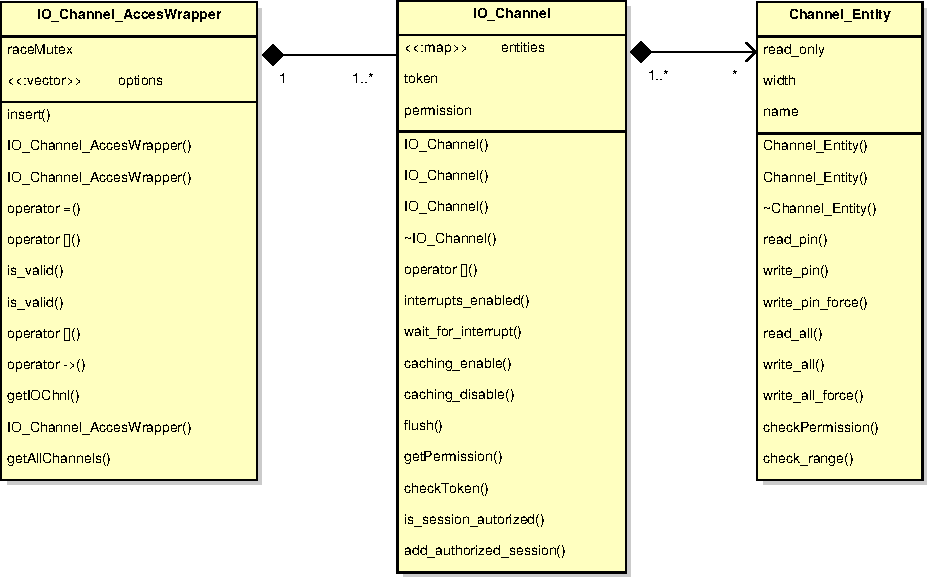
\includegraphics[width=0.95\textwidth ,clip]{./code/Aggregation.pdf}
		\caption{Klassendiagramm Aggregation der Klassen}
		\label{img:classAgregation}
	\end{center} 
\end{figure}	
Zu sehen ist die Aggregation zwischen dem \chphl{IO\_Channel\_AccessWrapper} den Kanälen \chphl{IO\_Channel} und den Entitäten \chphl{Channel\_Entity}. Alle Kanäle werden von dem  \chphl{IO\_Channel\_AccessWrapper} zusammengefasst. Ein Zugriff erfolgt ausschließlich über diesen Weg. 


\begin{figure}[H]
	\begin{center}
		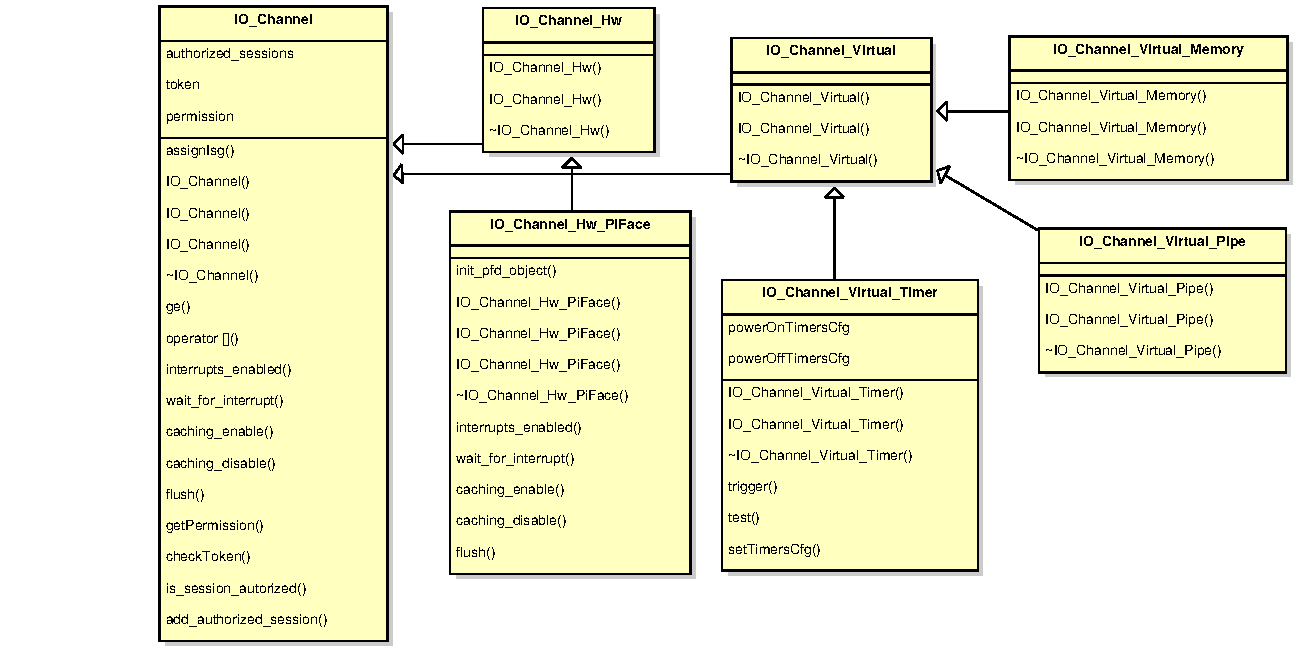
\includegraphics[width=0.95\textwidth ,clip]{./code/IOChannel.pdf}
		\caption{Vererbungshierarchie der Basisklasse IOChannel}
		\label{img:classIOChannel}
	\end{center} 
\end{figure}	

\begin{figure}[H]
	\begin{center}
		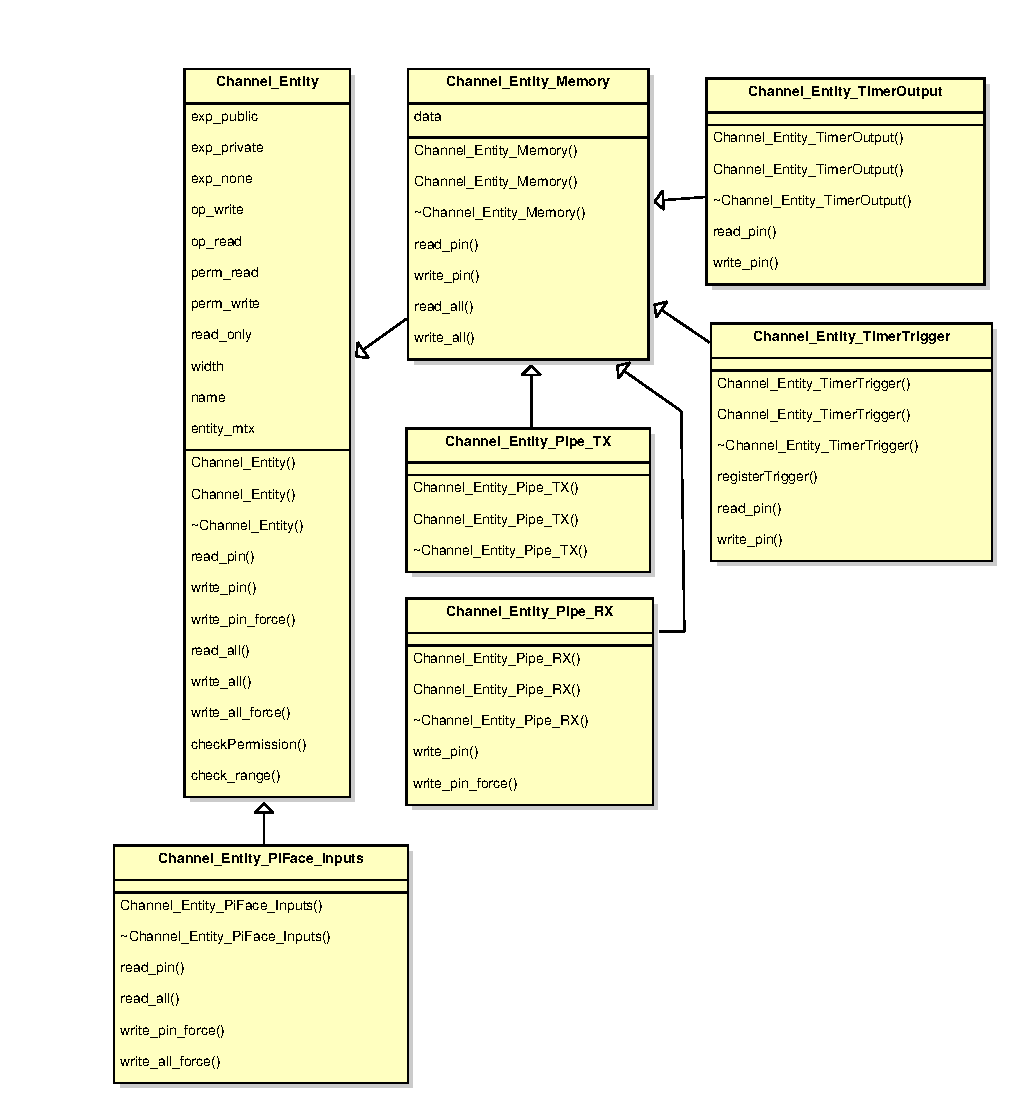
\includegraphics[width=0.95\textwidth ,clip]{./code/ChannelEntity.pdf}
		\caption{Vererbungshierarchie der Basisklasse ChannelEntity}
		\label{img:classChannelEntity}
	\end{center} 
\end{figure}	

Die Entitäten erben von der Basisklasse Entity. Sie überschreiben Methoden um lesend oder schreibend, entweder auf den gesamten Inhalt auf einmal oder Bitweise auf den Inhalt zuzugreifen. Dafür sind die Methoden read\_pin, write\_pin beziehungsweise read\_all und write\_all vorgesehen. 



\subsubsection{Hardware Kanäle}\label{kap:ums:hwchannels}
Der Wohl wichtigste Kanal ist der Hardware Kanal. Die Klassenstruktur in Abb. \ref{img:classIOChannel} zeigt, dass alle Kanäle eine gemeinsame Basisklasse haben. Der Hardware Kanal ist eine Spezialisierung der Basisklasse, welche spezifische Funktionen für die Entsprechende Hardware beherbergt. So finden sich hier Methoden zur Steuerung des Caching sowie ein blockierender Aufruf, welcher auf einen Interrput an der Hardware reagiert. Die Funktionen für den schreibenden und lesenden Zugriff auf die Ein- und Ausgänge der Hardware, sind in Entitäten gekapselt. Für eben jenen Zweck existieren zwei Spezialisierungen der \chphl{Channel\_Entity} (siehe Abb. \ref{img:classChannelEntity}) Basisklasse, welche für den Zugriff mit \chphl{i} für den Eingang (input) beziehungsweise \chphl{o} für den Ausgang (output) referenziert werden.   

\subsubsection{Merker Bausteine}\label{kap:ums:memorychannel}
Die erste Erweiterung, welche wie in Abb. \ref{code:chlnInit} zu sehen mit dem Buchstaben M referenziert wird, sind Memory Bausteine. Da ein Memory Baustein nicht richtungsorientiert sind, das heißt es existiert keine Eingangs oder Ausgangsgröße, wurde hier vom Benamsungsschema für Entitäten  abgewichen. Eine Referenzierung ist hier mittels eines oder mehrerer Buchstaben geplant. Somit bietet ein Merker Baustein Platz für 8 Zustandswerte pro verwendeter Entität. Bislang ist lediglich die Entität \chphl{a} angelegt, wobei geplant ist die Anzahl an Buchstaben beziehungsweise Entitäten durch einen Konstruktorparameter nach Außen zu führen, womit die Anzahl wie in Abb. \ref{code:chlnInit} zu sehen beim Einfügen bestimmt werden könnte, oder in einem weiteren Schritt in eine Konfigurationsdatei exportiert werden kann. 

\subsubsection{Timer Bausteine}\label{kap:ums:timerchannel}
Timer Bausteine waren die wohl komplexesten Bausteine. Eine Verzögerung im Programmablauf bedeutet entweder ein blockieren, was aber bedeuten würde, dass das Programm in dieser Zeit auch nichts anderes tun kann und somit nicht auf Ereignisse reagieren kann. Die andere alternative ist Multithreading, also das Einführen von Parallelen Handlungssträngen, welche weitere Probleme bringen. So muss zum Beispiel beim Zugriff auf gemeinsam genutzte Ressourcen dafür sorge getragen werden, dass nicht gelesen wird während gerade geschrieben wird. Des weiteren musste die Hauptschleife überarbeitet werden. Bislang wurde die Programmlogik bei jedem eintreten eines Hardware-Ereignisses genau einmal durchlaufen. Jedoch muss die Programmlogik nun auch durch Ablauf eines Timers erneut durchlaufen werden. Gelöst wurde dies mithilfe einer Binären Variable als Schalter, welche zusammen mit eines Mutex zur Vermeidung von gleichzeitigem Zugriff, und einer Condition Variable zur Benachrichtigung des Hauptprozesses, in die Klasse \chphl{iterationSwitchGuard} gekapselt wurde. 
Ein Timerbaustein (mehrere sind Theoretisch möglich), bietet 8 Konfigurierbare Timer. Dabei gibts es eine Entität um einen Timer auszulösen \chphl{t} (Trigger) und eine Entität, welcher als Ausgang fungiert \chphl{o} (Output). So ergibt sich in der Programmlogik die selbe Syntax, welche sich auch bei Hardwarekanälen bietet: Ein explarisches triggern des Timers 3 würde erfolgen, indem eine Zeile der Logikdatei mit \chphl{Tt3=} beginnt. Eine Verwendung des Ausgangswertes desselben Timers, würde durch integrieren des Bezeichners \chphl{[To3]} in die Logikzuweisung eines anderen Bezeichners erfolgen. Die Parametrisierung des Timers erfolgt durch einbinden einer Konfigurationsdatei (siehe Quellcode \ref{code:timersConf}) hierbei lassen sich für jeden Timer eine Einschaltverzögerung sowie eine Ausschaltverzögerung definiert werden. Jeder Wert ungleich null bewirkt eine Verzögerung, eine gleichzeitige Nutzung von Ein und Ausschaltverzögerung ist möglich. Werte gleich null bewirken eine sofortige Änderung am Ausgang, sobald sich der Eingangswert verändert. Beim Einlesen der Konfiguarionsdatei werden sämtliche Leerzeichen entfernt. Zudem kann mit einem Semikolon \chphl{;} oder einer Raute \chphl{\#} ein Kommentar eingeleitet werden, welches alle restlichen Zeichen der Zeile beim Einlesen entfernt. Die Verzögerungszeiten sind in Millisekunden anzugeben, wobei die Reihenfolge der nicht sukzessive erfolgen muss. Der Maximalwert beläuft sich auf 4.294.967.295, was die größte in unsignes long darstellbare Zahl ist und umgerechnet etwa 49 Tagen entspricht. 
\begin{listing}[H]
	\inputminted[numbersep=1pt,fontsize=\scriptsize,frame=single, firstline=14,lastline=25]{c}{./code/timers.conf}
	\caption{Beispiel der Timer Konfigurationsdatei}
	\label{code:timersConf}
\end{listing}


\subsubsection{Virtuelle Kanäle}\label{kap:ums:virtualchannel}
Virtuelle Kanäle sind ein Konzept dass die Kommunikation der Steuerung mit entfernten Endpunkten ermöglichen. Ein virtueller Kanal ist hierbei lediglich ein veränderter Memory Baustein, welcher entgegen entgegen anders als ein normaler Memory Baustein wieder richtungsorientiert ist. Das heißt es gibt eine Eingangs-Entität und eine Ausgangs-Entität. Hierbei muss beachtet werden, dass die Perspektive so gesetzt ist, dass ein Eingang die extern empfangenen Daten beinhaltet. Während in den Ausgang geschrieben wird. Die Gegenseite bildet der in \autoref{chp:ums:websockserver} beschriebene WebSocket Server, beziehungsweise was auch immer die Gegenseite bildet. Das kann die in Benutzeroberfläche dieses Projektes sein (siehe \autoref{chp:ums:JavaScriptFront}), oder auch jeder andere WebSocket fähige Client. Angedacht ist auch die Implementierung eines WebSocket Clients in das Backend, womit sich zwei Einheiten verbinden ließen. 


\subsection{Laden der Programmlogik aus Datei}\label{kap:ums:logicOutsource}
Das Logikprogramm wurde im nächsten Schritt in eine Textdatei ausgelagert. Sie soll künftig von der grafischen Benutzeroberfläche automatisch erstellt werden können, kann aber nach wie vor auch von Hand erstellt werden. Die Datei enthält einen Ausgang pro Zeile, gefolgt von einem Gleichheitszeichen und den Abhängigkeiten. Zeichen die auf ein Semikolon folgen, werden dabei als Kommentar gewertet und ausgelassen. Sie wird bei Programmstart eingelesen und verbleibt dann im Speicher. Zum Speichern der Daten wird ein \chphl{Vector} benutzt, welcher für jede Zeile der Logikdatei einen weiteren Eintrag erhält. Da vor einem Gleichheitszeichen lediglich ein Ausgang stehen darf (z.B. \ref{softLogic} Zeile 1: \chphl{Ho0}), ist somit jeder Eintrag des Vectors die Definition genau einer Abgeschlossenen Zuweisung. Bei Mehrfacher Definition eines Ausgangs, überschreibt die spätere Definition die vorangegangene. 

\begin{listing}[H]
	\inputminted[numbersep=1pt,fontsize=\scriptsize,frame=single, firstline=29,lastline=36]{c}{./code/logic.conf}
	\caption{Beispiel der Programmlogik Datei}
	\label{code:softLogic}
\end{listing}


\subsubsection{Erneutes Laden der Logik zur Laufzeit}\label{kap:ums:reloadConf}
Zum erneuten einlesen der Logik, wurde ein Signalhandler vorgesehen, welcher auf das Signal SIGUSR1 hört. Die entsprechende Funktion ließt dann die Logikdaten erneut ein und überschreibt damit die vorherige Version im Speicher. Damit muss die Steuerung nicht neu gestartet werden und ermöglicht das Steuerungsprogramm zur Laufzeit zu verändern.


\subsection{Hauptschleife und Iterationslogik}\label{kap:ums:mainloop}
Das Logikprogramm liegt nun im Speicher und das Programm betritt die Hauptschleife. Doch treibt ein einfaches polling die Auslastung des Prozessors unnötig nach oben. Nun könnte nach jedem Durchlauf eine gewisse Zeit gewartet werden, bevor eine neue beginnt. Doch das verringert die Reaktionszeit der Steuerung. Die beste Lösung findet sich direkt im Treiber des PiFaceDigital. Hier bietet sich eine Funktion, die bis zum Eintreten einer Veränderung der  Eingangswerte blockiert. Intern Eingesetzt wird hier ein Epoll, welcher einen File descriptor auf einen der GPIOs des Raspberry Pi überwacht und diesen somit als Interrupt Kanal nutzt. 


\subsection{Logik Prozessor}\label{kap:ums:logicProcessor}
Den Kern des Projektes bildet der in \autoref{code:logicEngine} gezeigte Logikprozessor. Es ist eine Methode, welche den in \autoref{kap:ums:logicOutsource} geladenen Logik-Vektor zeilenweise durchläuft. Im ersten Schritt wird die Zeile nun auf Vorhandensein eines Gleichheitszeichens hin überprüft (\autoref{code:logicEngine} Zeile \ref{codeline:split}). Eine Zeile ohne Gleichheitszeichen wird hierbei schlicht verworfen. Andernfalls wird zunächst der Teil vor dem Gleichheitszeichen näher untersucht. Dabei wird sichergestellt dass der Bezeichner aus drei Zeichen besteht, wobei die ersten beiden alphabetisch und der letzte numerisch sein muss. Diese drei Teile werden dann (Zeile \ref{codeline:charSeperateBegin}-\ref{codeline:charSeperateEnd}) für die weitere Verarbeitung gespeichert. Der fertig ausgewertete Teil nach dem Gleichheitszeichen, auf dessen Verarbeitung nachfolgend noch etwas genauer eingegangen wird und der nunmehr entweder \texttt{0} oder \texttt{1} ist, wird dem entsprechenden Kanal nun zugewiesen. Wie in \autoref{code:logicEngine} Zeile \ref{codeline:equation} zu sehen, wird nun eine Instanz \texttt{chnl} der Klasse \texttt{IO\_Channel\_AccessWrapper} für den eigentlichen Zugriff auf die Ressource verwendet. Zuvor müssen jedoch die vorher gespeicherten Teile des Bezeichners eingefügt werden verwendet. (Siehe \autoref{kap:ums:klassen}\chphl{ \nameref{kap:ums:klassen}}). 
Zudem wird dem Bezeichner in diesem Zuge ein Wert zugewiesen. Um diesen zu erhalten muss nun die Gleichung gelöst werden. Diese beinhaltet ebenfalls Bezeichner, welche vom Funktor \texttt{replaceIdentifier} durch dessen aktuellen Wert ersetzt wird. Zurück gegeben wird ein String, welcher nun nur noch aus Binärzahlen, arithmetischen Operatoren (\& für und bzw. | für oder) und Klammern besteht. Die eigentliche Lösung der Gleichung erfolgt dann mittels eines Funktionsaufrufes auf einen in Boost Spirit geschriebenen Parser (siehe Unterabschnitt \chpref{kap:ums:parsing}). 
\begin{listing}[H]

	\inputminted[numbersep=1pt,linenos=true, mathescape, numbers=left, fontsize=\scriptsize,frame=single, firstline=186,lastline=222]{c}{./code/main-klassenstruktur.cpp}
	\caption{Logik Engine}
	\label{code:logicEngine}
\end{listing}
\subsection{WebSocket Server}\label{chp:ums:websockserver}
\subsubsection{Basis}
Um die Steuerung mit der Außenwelt zu Verbinden wurde ein WebSocket (siehe \ref{chp:grdlgn:webSocket}) Server in das Backend integriert. Als Basis hierfür diente das Beispiel, welches von Vinnie Falco im  Rahmen eines Vortrages auf der \texttt{CppCon 2018} erstellt wurde \cite{URL:WebSocketCppCon}. Die Funktion dieses Beispiels ist das Bereitstellen  eines WebSocket Chatservers. Dieser baut auf einem rudimentären HTTP Server auf und ist deshalb in der Lage auch normale HTTP Anfragen zu beantworten. Auf diesem Wege erhält der Webbrowser des Clients die HTML Webseite, in welche gleichzeitig auch der JavaScript Chat-Client enthalten ist der letztendlich die direkte Verbindung zum WebSocket Server aufbaut. Nachdem die Verbindung erfolgreich herstellt wurde, kann der Benutzer Texteingaben tätigen und diese an den Server senden, welcher diese dann an alle verbunden Clients verteilt. Da es nun relativ einfach umsetzbar ist, anstatt Text auch andere Formate wie etwa JSON über diesen Server an die Clients zu senden, schien dieses Beispiel eine ideale Grundlage zu sein. So könnte anstatt Text ein JSON mit dem Status der Ein- und Ausgänge der Steuerung an die verbundenen Clients verteilt werden, welche diese dann mit einer JavaScript Anwendung so umsetzen, dass der Status der Ein- und Ausgänge visuell dargestellt werden. Zudem ist über diesen Kommunikationskanal auch ein Schreibzugriff denkbar. So könnte ein symbolisch dargestellter Schalter im Frontend beim Anklicken per JavaScript Funktion einen Befehl an das Backend senden, welches diesen dann ausführt. 
\subsubsection{Erweiterung}
Das vorher erwähnte Beispiel wurde in einem ersten Schritt in einen Unterordner des Projektes verschoben und das CMake-File dahingehend geändert, das anstatt eines eigenen Executables eine Library gebaut wird, welche dann vom Grundprojekt verwendet wird. Das Unterprojekt wurde zudem als Abhängigkeit deklariert sodass es beim bauen des Hauptprojektes automatisch neu gebaut wird, sofern sich Änderungen im Unterprojekt ergeben haben. Die einfachste Erweiterung war es, die schon vorhandene \texttt{broadcast} Funktion zu verwenden, um bei einer Änderung an den Ein- und Ausgängen eine Nachricht an alle verbundenen Clients zu senden. Da jedoch immer nur eine Nachricht gleichzeitig gesendet werden kann, wurde eine \texttt{Queue} verwendet, welche die Nachrichten sammelt, und diese dann  nacheinander zustellt. Im nächsten Schritt wurden eingehende Nachrichten nun nicht mehr bloß eins zu eins an die \texttt{broadcast} Methode übergeben, und damit an alle Clients weitergeleitet. Stattdessen mündeten diese nun in eine weitere \texttt{Queue}: \chphl{Command-Queue}. Eingehende Nachrichten sollen damit gesammelt werden um die darin enthaltenen Befehle auszuführen.
\subsubsection{Zugriffsbeschränkung}\label{chp:ums:websock:auth}
Um zu verhindern das jeder Client nun unkontrolliert vollen Zugriff auf alle Kanäle der Steuerung erhält, wurde daraufhin ein Konzept für die Zugriffsbeschränkung erarbeitet. Dafür wurden zwei Benutzerrollen eingeführt. \texttt{public} und \texttt{private}. Sie gelten für jeden Kanal und jeden Client individuell. Dafür besitzt jeder Kanal ein \texttt{private\_token}. Authentifiziert sich ein Benutzer mittels \texttt{auth:<Kanal>:<Token>} für den Kanal, so wechselt er für diesen Kanal in die Rolle \texttt{private}. Da jeder Kanal aus mehreren Entitäten besteht, besitzt nun jede dieser Entitäten die Eigenschaften \texttt{expose\_read} und \texttt{expose\_write}. Zulässige Werte hierfür sind jeweils \texttt{public} \texttt{private} oder \texttt{none}. Bei Zugriff auf den Kanal bzw. die Entität wird nun darauf geprüft ob der Benutzter \textbf{mindestens} die eingetragene Berechtigung hat. Nehmen wir zum Beispiel den Kanal Hardware \chphl{H}. Dessen Entitäten \texttt{i} für die Eingänge und \texttt{o} für die Ausgänge haben beide \texttt{expose\_read} auf \texttt{private} gesetzt. Das \texttt{private\_token} ist mit \texttt{top-secret-123} definiert. Ein Verbundener Client müsste sich nun erst mit dem Befehl \texttt{auth:H:top-secret-123} für den Kanal authentifizieren, bevor er Statusinformationen über die Entitäten dieses Kanals erhält. Wäre \texttt{expose\_read} auf \texttt{public} gesetzt, würde er diese Informationen ohne vorherige Authentifikation erhalten. Anders herum, würde derr wert \texttt{none} bedeuten, dass niemand - nicht einmal ein Authentifizierter Client - Statusinformationen zu dieser Entität erhält. Quellcode \ref{code:Jsonresponse} stellt ein typisches Statusupdate der privaten Entitäten \texttt{Qo} und \texttt{Qi} dar, darauf folgt das Update aller Entitäten, die als \texttt{public} definiert wurden.  
\begin{code}
	\captionof{listing}{JSON Status Update von privaten und öffentlichen Entitäten}
	\label{code:Jsonresponse}
\begin{minted}
	[
	frame=lines,
	framesep=2mm,
	baselinestretch=1.2,
	fontsize=\footnotesize,
	linenos
	]
	{c}
{"Qo" : 4, "Qi" : 1}
{"Po" : 170, "Pi" : 4, "Ho" : 0, "Hi" : 6}
\end{minted}
\end{code}

\subsection{Benutzeroberfläche}
Die Benutzeroberfläche ist bei diesem Projekt in Form von einer Webseite umgesetzt, welche über einen Internetbrowser aufgerufen werden kann.  Wie in \autoref{img:externalAccess} zu sehen, dient hierfür die IP Adresse oder der Hostname der Steuerung solange man sich im selben Netzwerk befindet. Andernfalls muß der Internetrouter für einen ein externen zugriff eingerichtet werden. 
 \begin{figure}[H]
	\begin{center}
		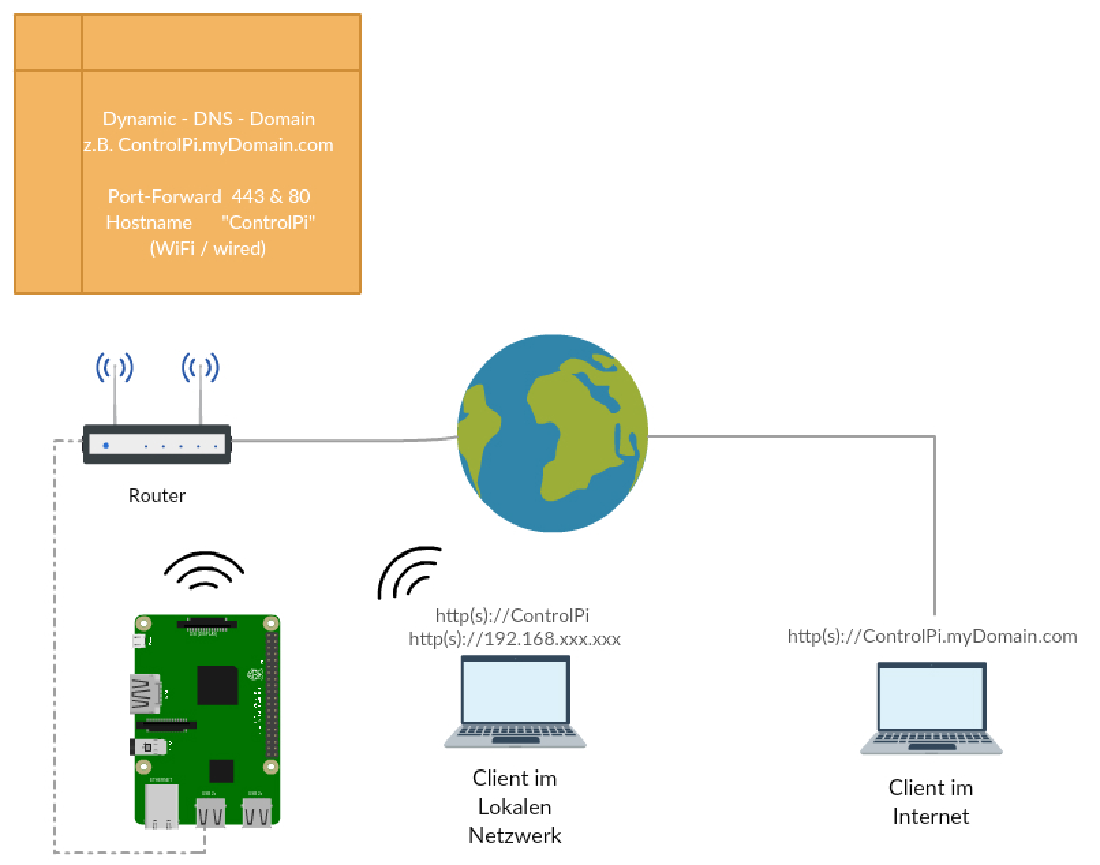
\includegraphics[width=0.75\textwidth ,clip]{./images/IFTTT.pdf}
		\caption{Zugriff auf die Weboberfläche}
		\label{img:externalAccess}
	\end{center} 
\end{figure}

\subsubsection{Übersicht Komponenten}
Die eigentliche Anwendung ist Hauptsächlich in HTML und JavaScript geschrieben und wird im Browser des Benutzers ausgeführt. Um die Benutzeroberfläche mit dem Rest der Anwendung kommunizieren zu lassen, bedarf es mehrerer Komponenten. \autoref{img:externalNetworking} zeigt diese und illustriert die Zusammenhänge. Obwohl der Hauptteil der Anwendung über JavaScript Websockets eine direkte Verbindung vom Browser zum Backend herstellen könnte, wird als direkte Schnittstelle zum Browser ein Apache2 Webserver eingesetzt. Dieser wird um das Proxy-Modul modproxy erweitert was es ermöglicht an das Backend gerichtete Anfragen mit dem WebSocket Header auf die lokale loopback Adresse \texttt{127.0.0.1} weiterzuleiten, während alle sonstigen Anfragen vom Webserver direkt beantwortet werden können. Zum einen wird hierdurch die Konfiguration von Verschlüsselten Verbindungen über SSL und den Abruf der dazu nötigen Zertifikate erheblich vereinfacht, denn einige Zertifizierungs-Anbieter wie zum Beispiel Let's Encrypt *REF* bieten extra auf Apache zugeschnittene Scripte, die ebendies fast vollständig Automatisieren. Zum anderen ist es so möglich die Auslieferung der HTML und JavaScript Quellen an den Webserver zu delegieren, anstatt bei einer eigenen Implementierung Sicherheitslücken und Performance-Probleme zu riskieren. Weiterhin ermöglicht es dieser Ansatz auch PHP Scripte zu verarbeiten, dies wird zum Beispiel eingesetzt um Konfigurationsdateien vom Browser auf dem Server abzulegen, oder durch dem Backend Signale zu senden wenn es die Logikdatei erneut einlesen soll.

\begin{figure}[H]
	\begin{center}
		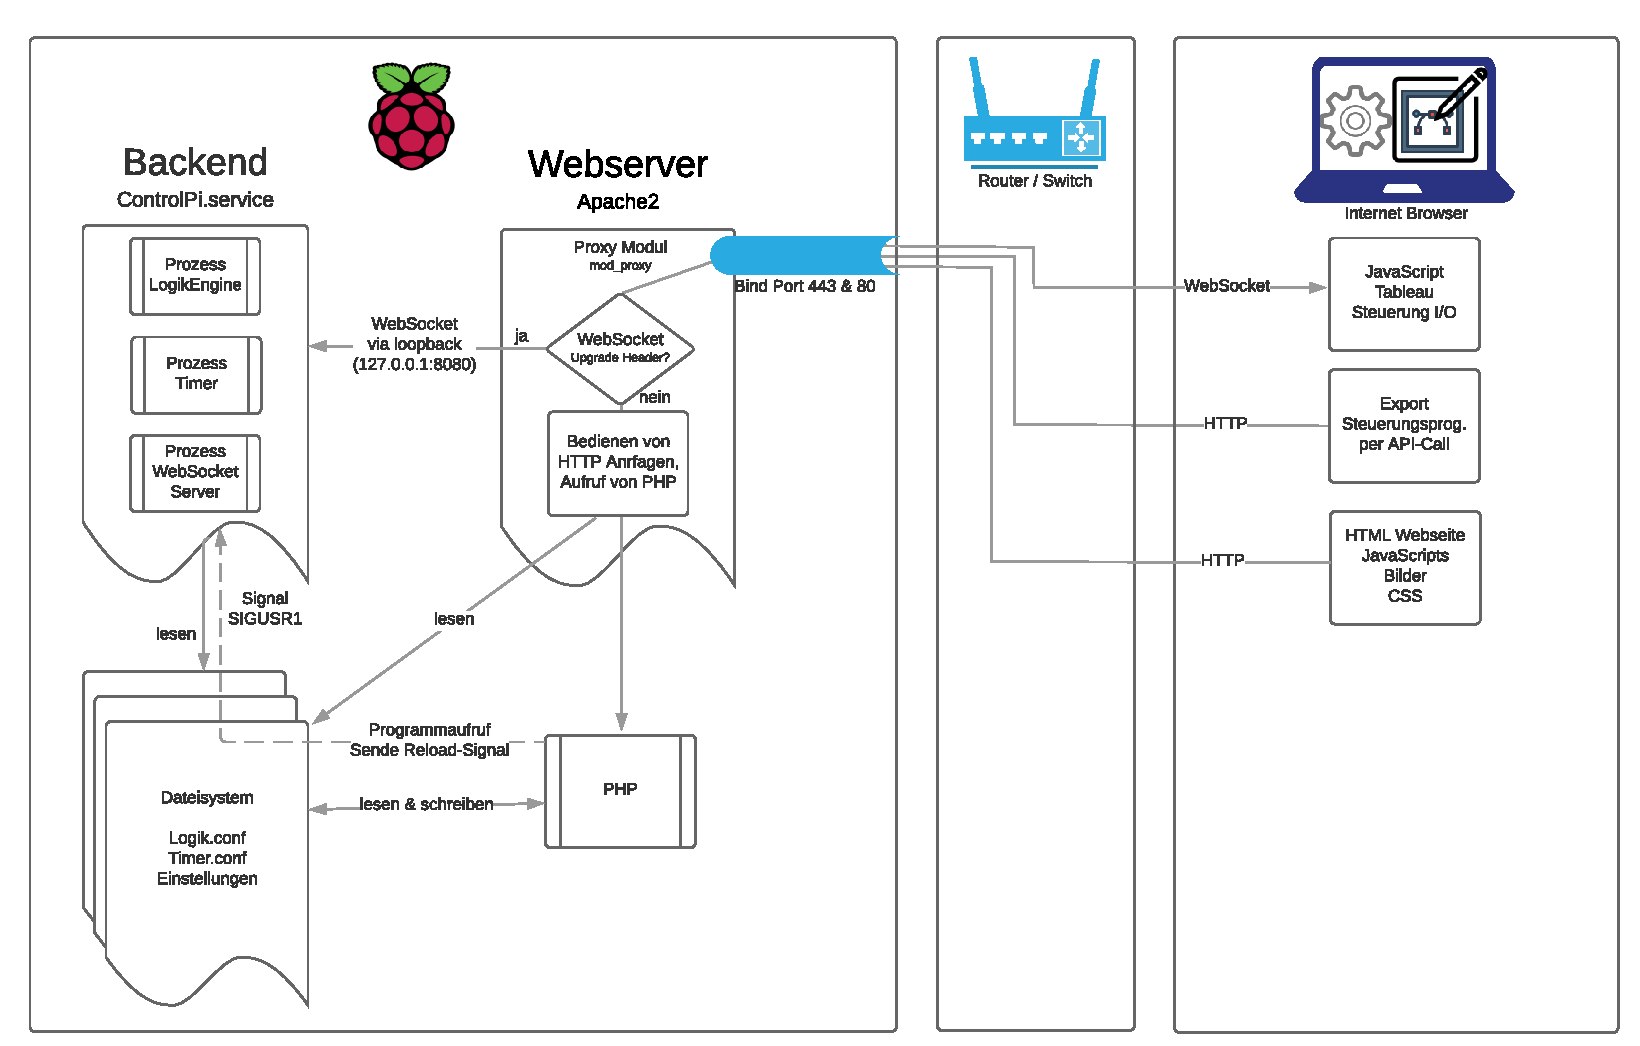
\includegraphics[width=0.9\textwidth ,clip]{./images/BackendFrontend.pdf}
		\caption{Networking Übersicht}
		\label{img:externalNetworking}
	\end{center} 
\end{figure}
\subsubsection{Apache Webserver}
\todo{Was schreiben?!}

\subsubsection{JavaScript Anwendung}\label{chp:ums:JavaScriptFront}
Um den Status der Steuerung auch sehen zu können, wenn man sich nicht in Sichtweite befindet, wurde hierzu eine Übersicht in die Benutzeroberfläche implementiert. \autoref{chp:FrontendUebersicht}

\subsubsection{Logik Editor CircuitVerse}\label{kap:circuitVerse}
Die Wahl für einen Graphischen Logikeditor fiel auf den mit der MIT Lizenz gekennzeichneten Editor CircuitVerse *REF*. Die Lizenzierung gestattet es, das Programm zu verändern und weiter zu verbreiten. Der in \autoref{img:circuitVerseBasic} gezeigte Screenshot, zeigt den Aufbau des Editors. Im linken Abschnitt kann dabei zwischen verschiedenen Bauteilen gewählt werden, welche dann per Drag \& Drop auf die rechts daneben befindliche Zeichenfläche gezogen werden können. Grüne Punkte kennzeichnen dabei die Anschlussknoten, welche dann wiederum durch ziehen mit gehaltener linker Maustaste miteinander verbunden werden können. CircuitVerse bietet überdies die Möglichkeit, die erstellte Zeichnung in einem eigenen Format zu  speichern, sowie sie als Grafik zu exportieren. Des weiteren gibt es die Möglichkeit eine Zeichnung anhand einer Logiktabelle automatisch erstellen zu lassen. 

\begin{figure}[H]
	\begin{center}
		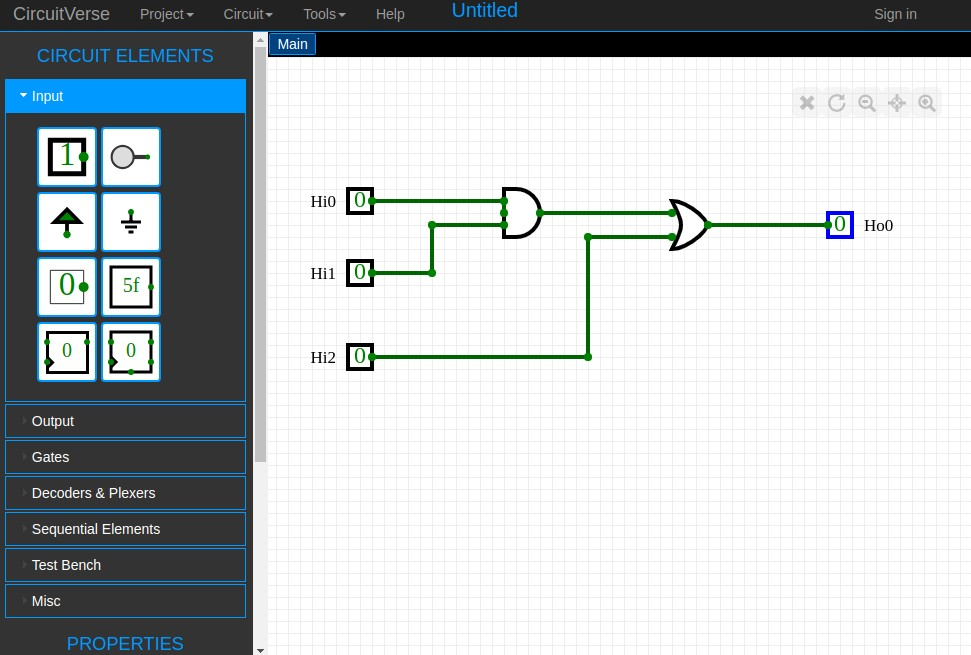
\includegraphics[width=0.65\textwidth ,clip]{./images/circuitverse.jpg}
		\caption{Screenshot einer Logikschaltung in CircuitVerse}
		\label{img:circuitVerseBasic}
	\end{center} 
\end{figure}	

\paragraph{Erweiterung für den Export}\label{par:erw}
 Eine Erweiterung von CircuitVerse ist nötig, um die gezeichnete Logikschaltung in ein Format umwandeln zu können, welches vom Backend verstanden wird. Weiterhin muss das Benamsungsschema (siehe \chpref{kap:ums:banamsung}) eingebracht werden. Letztlich muss auch die Bauteile-Auswahl auf jene Bauteile reduziert werden, welche auch tatsächlich in der Steuerung verfügbar sind. \chpref{kap:ums:logicOutsource} beschriebt das Format der Datei, die letztlich aus einer gezeichneten Logikschaltung gewonnen werden soll. CircuitVerse verwendet für die Speicherung der Schaltung eine JSON-Struktur. Dabei wird in Bauteile und Knoten unterschieden. Ein Bauteil hat ein oder mehrere Knoten. Wobei Knoten miteinander verbunden werden können, und dann jeweils Informationen über angeschlossene Knoten enthalten. \autoref{img:circuitVerseNodes} verdeutlicht, wie CircuitVerse die Knoten verwendet. Die Grundlage für die Abbildung ist ein Grafikexport von CircuitVerse, wobei die Knotennummern zum besseren Verständnis der Funktionsweise besonders gekennzeichnet wurden. In \chphl{ \autoref{img:circuitVerseJson} \nameref{img:circuitVerseJson}}ist die zugehörige JSON-Datenstruktur abgebildet.
 \begin{figure}[H]
 	\begin{center}
 		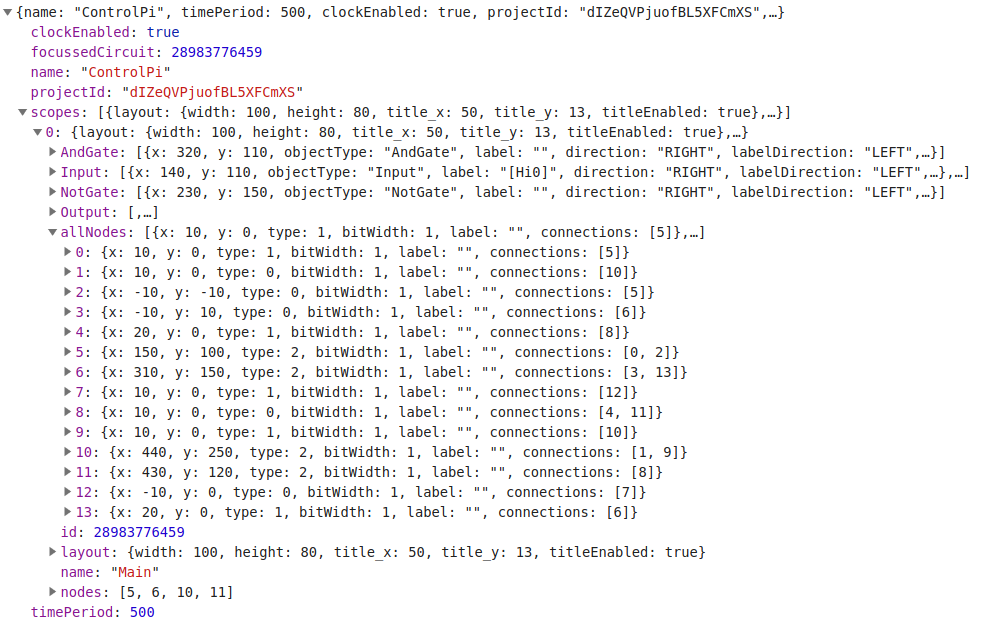
\includegraphics[width=0.8\textwidth ,clip]{./images/circuitverseLogicJson.png}
 		\caption{Darstellung der JSON Datenstruktur}
 		\label{img:circuitVerseJson}
 	\end{center} 
 \end{figure}	
 
 \begin{figure}[H]
 	\begin{center}
 		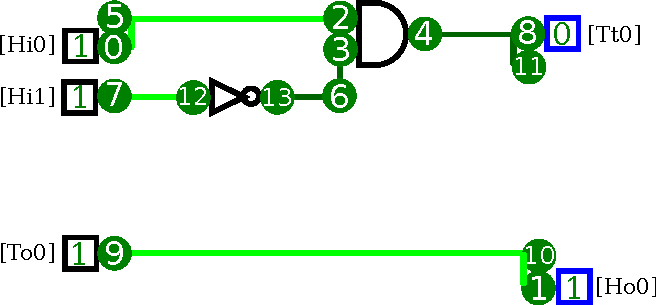
\includegraphics[width=0.65\textwidth ,clip]{./images/circuitverseLogicNodes.pdf}
 		\caption{Logikschaltung mit gekennzeichneten Knoten}
 		\label{img:circuitVerseNodes}
 	\end{center} 
 \end{figure}	
 
 
 In der vorangehenden Abbildung \ref{img:circuitVerseNodes} ist zu sehen, dass jedes Bauteil einen oder mehrere Knoten Besitzt. In \autoref{img:circuitVerseJson} ist zu sehen, dass jeder dieser Knoten eine eigene Zeile unterhalb von \texttt{allNodes} besitzt. Hieraus geht hervor, mit welchen anderen Knoten er verbunden ist. Außerdem verbirgt sich im Feld \texttt{Typ}, die Information ob es sich um einen Ausgangsknoten einen Eingangsknoten oder einen Verbindungsknoten handelt. Ist der Knoten vom Typ Eingangknoten oder vom Typ Ausgangsknoten so gehört er einem Bauteil wie einem Logikgatter, einem Eingangsbausteinen oder einem Ausgangsbausteinen. Die Anordnung der Knoten ist logischer weise anders herum wie die der Bauteile, so besitzt ein Ausgangsbaustein genau einen Eingangsknoten (z.B.  \ref{img:circuitVerseNodes} Knoten 1), sowie ein Eingangsbaustein über einen Ausgangsknoten verfügt (z.B. \autoref{img:circuitVerseNodes} Knoten 9). Ein Gatter hingegen hat einen Ausgangsknoten sowie einen oder mehrere Eingangsknoten. (z.B. \autoref{img:circuitVerseNodes} Eingangssknoten 3,4 und Ausgangsknoten 4) Für die Umwandlung in Textform schien es am sinnvollsten an einem Ausgang anzusetzen und eine Wegfindung durchzuführen, welche beim Erreichen eines Eingangsbausteins einen Endpunkt hat. Dazu durchläuft der in \autoref{img:circuitVersePAP} gezeigte rekursive Algorithmus den Weg von einem Ausgangsknoten bis zu einem Eingangsknoten. Ist ein Eingangsknoten erreicht, so wird geprüft ob es sich um den Ausgang eines Eingangsbausteins handelt, oder um den Ausgang eines Logikgatters. Da CircuitVerse die Knoten jedoch nicht nach der Art des zugehörigen Bauteils, sondern nur in Eingangsknoten Ausgangsknoten oder Leitungsknoten unterteilt, muss die in \ref{img:circuitVerseJson} gezeigte Struktur oberhalb der Eigenschaft \texttt{allNodes} vorab durchlaufen werden. Hierbei wird ein Lookup Array angelegt (siehe \autoref{img:circuitVerseLookup}), welches die Bauteile mit der Knotennummer ihres Ausgangs indiziert. Bezogen auf das in \autoref{img:circuitVerseNodes} gezeigte Beispiel, würde für das AND-Gate ein Eintrag mit dem Index 4 angelegt. \autoref{img:circuitVerseLookup} Zeigt den Eintrag für dieses AND-Gate in der aufgeklappten Zeile mit dem Index \texttt{4}. Das Array \texttt{nodesIn} beinhaltet die Knoten 2 und 3. An diesem Punkt, ruft die Funktion zur Wegfindung sich nun selbst auf. Auf diese weise werden sämtliche Logikgatter durchlaufen. In diesem Beispiel (siehe \autoref{img:circuitVerseNodes}) würde die Wegfindung von Knoten 2 über Knoten 5 auf Knoten 0 Treffen. Dieser ist jedoch kein Gateknoten sondern der Knoten eines Eingangsbausteines: Ein Endpunkt ist erreicht, das heißt es wird nun die Zeichenkette \texttt{[Hi0]} zurückgegeben. Zurück im vorher besprochenen AND-Gate, wird diese Zeichenkette nun mit dem Rückgabewert des Stranges an Knoten 3 und einem Kaufmännischen und (\&) verkettet. Da das And Gate genau zwei Eingangsknoten hat, sind nunmehr alle Knoten abgearbeitet und der Baustein gibt die Zeichenkette \texttt{[Hi0] \& ![Hi1]} zurück. Im Eingangsknoten wird diese Zeichenkette nun um den Bezeichner ergänzt.  Somit ergibt sich \texttt{[Tt0]=[Hi0] \& ![Hi1]} als Gesamtergebnis. 
  \begin{figure}[H]
 	\begin{center}
 		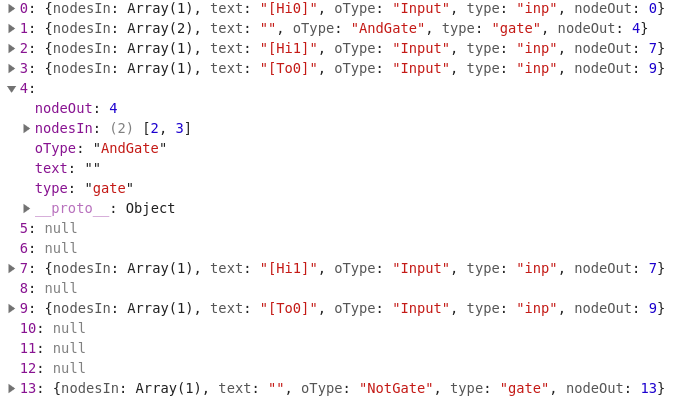
\includegraphics[width=0.65\textwidth ,clip]{./images/circuitverseLookup.png}
 		\caption{Lookup Array}
 		\label{img:circuitVerseLookup}
 	\end{center} 
 \end{figure}	
 
   \begin{figure}[H]
 	\begin{center}
 		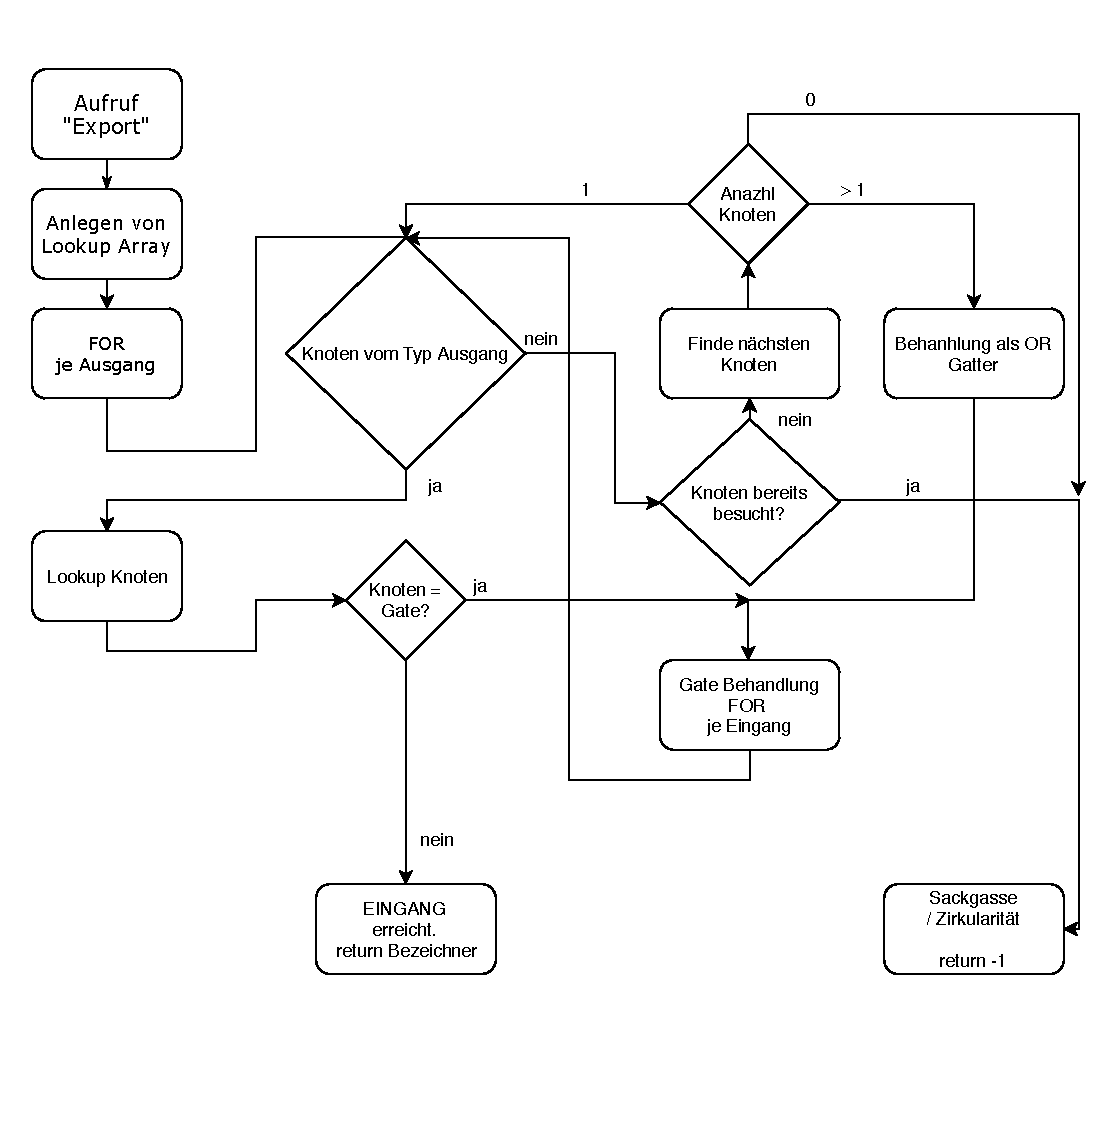
\includegraphics[width=0.75\textwidth ,clip]{./images/PAP7.pdf}
 		\caption{Programm Ablaufplan}
 		\label{img:circuitVersePAP}
 	\end{center} 
 \end{figure}
 
 \paragraph {Anpassung der Eingangsbausteine}
 
 Wie in \chphl{\ref{par:erw} \nameref{par:erw}} besprochen, wurde CircuitVerse um einen Algorithmus zum Export der gezeichneten Schaltung erweitert. Dieser wird über einen neuen Menüpunkt (siehe \ref{img:circuitVerseBright}) gestartet und zeigt dann wie in \autoref{img:circuitVerseBrightPrompt} zu sehen, das Exportergebnis zur Überprüfung an. Nach der Bestätigung des Ergebnisses wird dieses per Ajax Aufruf an ein in \autoref{kap:ums:adapterphp} näher beschriebenes PHP Script übergeben, welches es dann als Textdatei speichert. Der Menüpunkt \texttt{Save Online} schreibt das bisherig verwendete JSON Format über die selbe Schnittstelle in eine weitere Textdatei auf dem Server. Dabei wird zudem eine Abbildung der Schaltung erzeugt und ebenfalls auf den Server übertragen. Letztlich dient die Schnittstelle auch dem lesenden Zugriff auf die JSON-Datei. Sie wird beim ersten Aufruf des Logikeditors somit vom Server heruntergeladen. Damit kann die bereits vorhandene Steuerung erweitert oder verändert werden. Um zu vermeiden dass sich die Logik in der JSON Datei von der Logik in der vom Backend lesbaren Logikdatei unterscheidet, soll die Speicherung in einen Menüpunkt zusammengeführt werden. Dies dient vor allem auch dem einfacheren Verständnis durch den Endbenutzer. Es schränkt jedoch die Möglichkeit ein, neben der Steuerung die gerade \gqq{in Betrieb} ist, weitere alternative Steuerungsprogramme abzuspeichern.

\begin{figure}[H]
	\begin{center}
		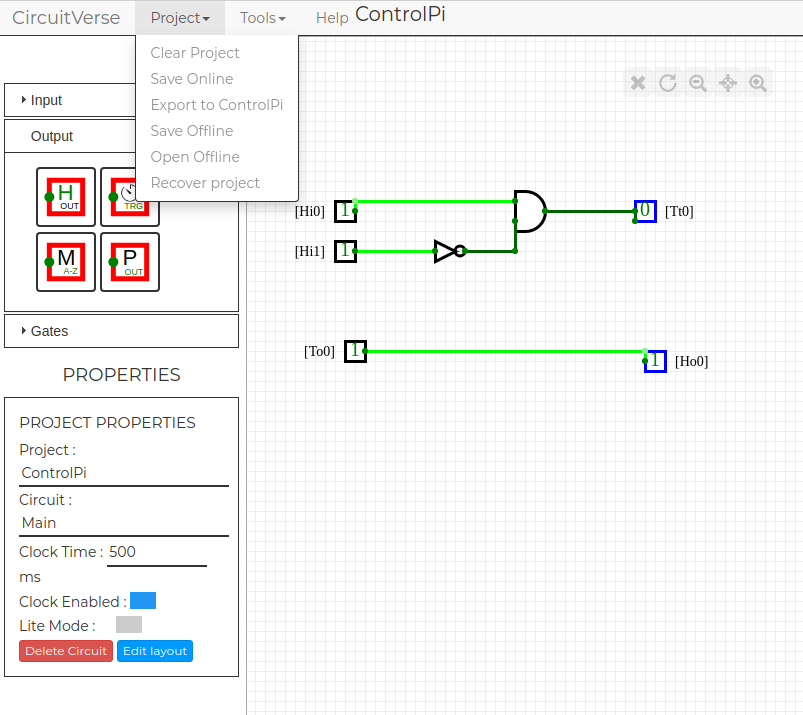
\includegraphics[width=0.75\textwidth ,clip]{./images/circuitverseLogicBright.png}
		\caption{Umgestatletes CircuitVerse}
		\label{img:circuitVerseBright}
	\end{center} 
\end{figure}

\begin{figure}[H]
	\begin{center}
		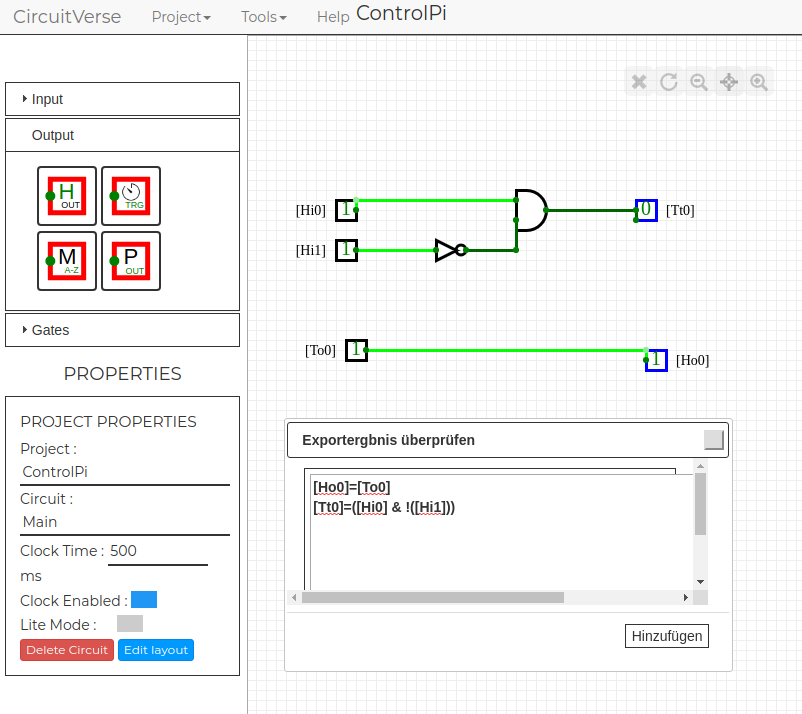
\includegraphics[width=0.75\textwidth ,clip]{./images/circuitverseLogicBrightPrompt.png}
		\caption{Dialog mit Exportergebnis}
		\label{img:circuitVerseBrightPrompt}
	\end{center} 
\end{figure}




\subsubsection{PHP Adapter Programme}\label{kap:ums:adapterphp}
\paragraph{Schnittstelle zum Speichern als Datei}\label{par:saveFile}
Da CiruitVerse als JavaScript Anwendung im Browser ausgeführt wird und somit keinen direkten Zugriff auf das Dateisystem des Servers hat, ruft es beim Speichern oder beim Laden per Ajax eine URL auf. Um Dateien nun persistent in das Dateisystem des Servers ablegen zu können wird eine API Schnittstelle benötigt, welche über ein rudimentäres PHP-Skript \texttt{logicUpdateApi} realisiert wurde. 
Dies geschieht über ein anderes PHP Skript, welches  ebenfalls über eine Ajax Anfrage angesprochen wird. Außerdem ließt dieses Script ebendiese Datei, wenn es beim Laden dieser CircuitVerse Version über JavaScript mittels Ajax aufgerufen wird. Zwischen lesendem und schreibendem Zugriff wird über die Verwendete Zugriffsmethode unterschieden, wobei \texttt{POST} einen schreibenden Zugriff gewährt und \texttt{GET} den Inhalt der Datei ließt. Da der Logikeditor in ein Helles Template eingebettet werden soll, wurde außerdem das Farbschema und die Schriftart modifiziert. 

\paragraph{WebSocket Adapter}
Das im letzen Abschnitt \ref {par:saveFile} beschrieben Verfahren zum Ablegen von Konfigurationsdaten ist ein einmaliges Ereignis, dementsprechend wird hier auch eine normale HTTP Anfrage eingesetzt, welche nach vollständiger Übertragung abgebaut wird. Im Unterschied dazu wird für die Ansteuerung der Virtuellen Kanäle sowie für die Statusabfrage der Phsyikalischen Ein und Ausgänge eine persistente Verbindung aufgebaut. Dabei baut der Client eine Verbindung zu dem WebSocker Server auf welcher in Kapitel \ref{chp:ums:websockserver} näher beschrieben wird. Um duch einmalige Ereignisse von externen Diensten per HTTP zu ermöglichen, baut ein PHP Script nun \texttt{on-demand} eine WebSocket Verbindung zu dem im Backend \ref{chp:grundl:backend} integrierten Server auf, setzt den gewünschten Befehl um und baut die Verbindung daraufhin wieder ab. 

\subsubsection{IFTTT}
Um eine Anbindung an IFTTT zu ermöglichen, bieten sich WebHooks an. Hierbei wird beim Auslösen eines Ereignisses eine vorher hinterlegte URL aufgerufen. Im Falle dieses Projekts, wird als Ziel hierfür die URL eines PHP Scripts verwendet, welches dann kurzzeitig eine WebSocket Session zum Backend herstellt und diese nach der vollständigen Übermittlung der Daten wieder Abbaut. Dabei dient ein Array in der Parameterliste dazu, beliebig viele Befehle mitzugeben, welche dann sequentiell über den WebSocket Kanal gesendet werden. Ein Beispiel wäre, dass nach dem Herstellen der Verbindung durch die Übermittlung des Authentifizierungs-Token der Schreibzugriff für die Ressource erworben wird, um durch einen weiten Befehl schreibend auf die Ressource zuzugreifen. Als Auslöser kann ein beliebiger anderer IFTTT Service dienen. Im einfachsten Fall wäre dies ein Button für den Smartphone-Homescreen.  



\clearpage


